\section{Methodology}
\subsection{Adversarial Assumptions}
There are a few assumptions that are made about the supposed attacker in the simulation scenario.  The first assumption is that the attacker is connected wirelessly to the target node. Another assumption is that the attacker has knowledge about the node they are attacking. The attackers goal in this scenario is to consume enough of the power from the target node so that the node is no longer able to transmit packages.  Another assumption is that the attacker has the capabilities to send a high volume of packets very quickly to the target node.
\subsection{Target Assumptions}
The target node similarly has assumptions associated with it in the simulation.  We assume that the node is a wireless sensor node connected to other wireless sensor nodes.  We also assume that the most power in the node is allocated to transmission, with reception being second.  We assume that the target node has limited power to allocate to each of its functions.
\subsection{Simulation Setup}
We are using NS3 to simulate two wireless nodes connected to each other. We are simulating two different kinds of attacks on the target node. The first attack is one in which many packets are sent rapidly from the attacker node to the target node in order to force the target node to accept a multitude of transmissions and drain its battery as shown in the figure below. 

\begin{figure}[h!]
\centering
\maketitle{Adversarial Game 1}
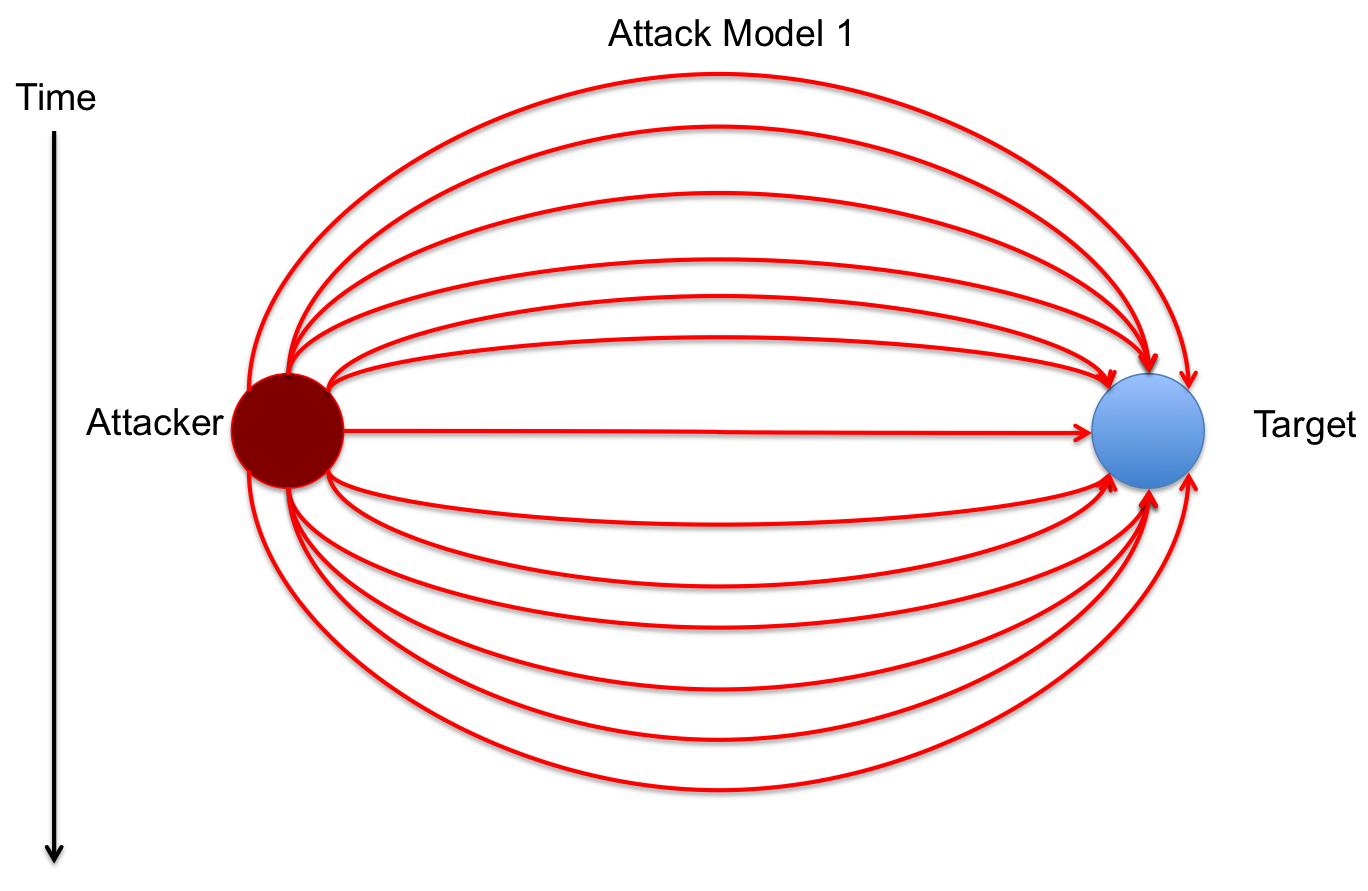
\includegraphics[width=\linewidth]{Figures/AModel1.png}
\caption{The figure above depicts an attacker continually bombarding a node with packets which force the target node to do calculations and thereyby conttributes to the draining of the initial energy supply.}
\end{figure}

The second attack is one in which the attacker node requests a transmission from the target node but then does not send any acknowledgements. This attack forces the target node to use power trying to send (many times) a succesful transmission but never is able. This results in the target node slowly being drained of power while transmitting it is diagramed below. 

\begin{figure}[h!]
\centering
\maketitle{Adversarial Game 2}
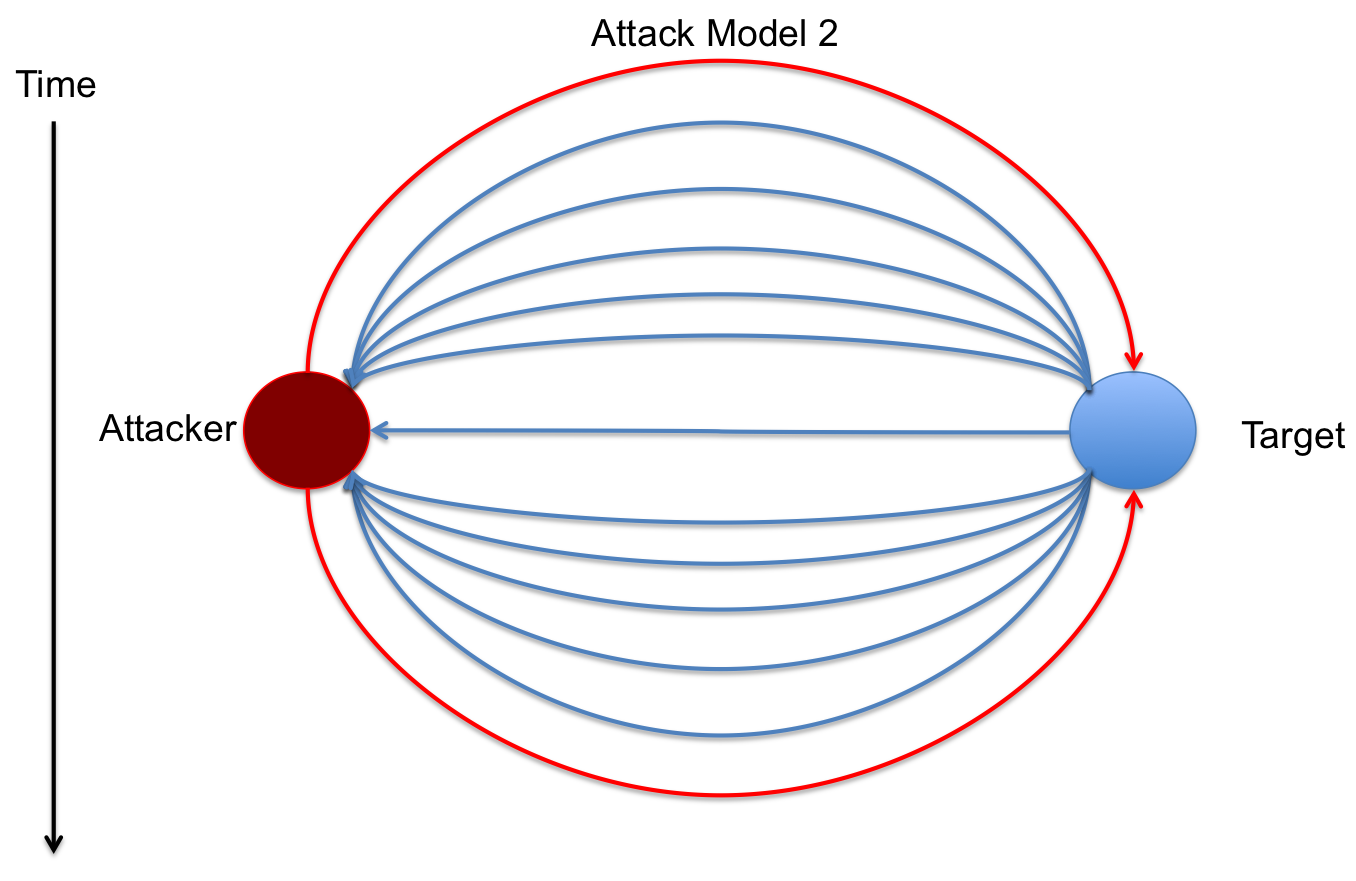
\includegraphics[width=\linewidth]{Figures/AModel2.png}
\caption{The figure above depicts an attacker requesting a transmission from a node with forces the target node to send the message over and over (because the attacker doesn't send an acknowledgement for a long time) conttributes to the draining of the initial energy supply.}
\end{figure}


For the purpose of simplicity and to limit variables we are modeling two nodes, an attacker and a target, as opposed to a large network of nodes. When setting up the model we have multiple variables that we concern ourselves with that can affect the simulation. The most important variables are the battery size of the target node, the number of packets being sent from the attacker to the target, and the time interval at which the attacker sends the packets. Other variables include distance between the two nodes and the size of each packet. The simulation creates two nodes that are both assigned an ipv4 address and connects them together via WiFi. The simulation then runs the specified attack with the variables that it were assigned. While packets are being transferred the simulation prints out data after each successful transmission. The data printed is the amount of battery left before and after the packet is sent and received and the time stamp at which the packet was transmitted by the attacker node and received by the target node. The simulation ends when the target node no longer has enough power to receive packets.
